\section[Sistema Eletrônico] {Sistema Eletrônico}
A parte eletrônica do projeto é dividida em duas categorias: sistema de controle e sistema de comunicação. O sistema de controle é responsável pela movimentação do atuador linear e acionamento do eletroímã. Já a parte de sistema de comunicação, ficará responsável por toda comunicação entre o banco de dados (servidor) e o atuador.

\subsection{Dispositivo Raspberry PI}
É o principal dispositivo para o funcionamento do sistema de controle e de comunicação, é um computador de baixo custo do tamanho de um cartão de crédito onde tem um poder de processamento bem eficiente para cumprir tudo que o projeto necessita. Este computador, em termos gerais, fará a comunicação entre o pedido do livro, feito pelo usuário, e o funcionamento do atuador para apanhar o livro requisitado na estante. O modelo usado neste trabalho será a Raspberry PI 3. Abaixo é apresentada algumas especificações.

\begin{figure}[!h]
\centering
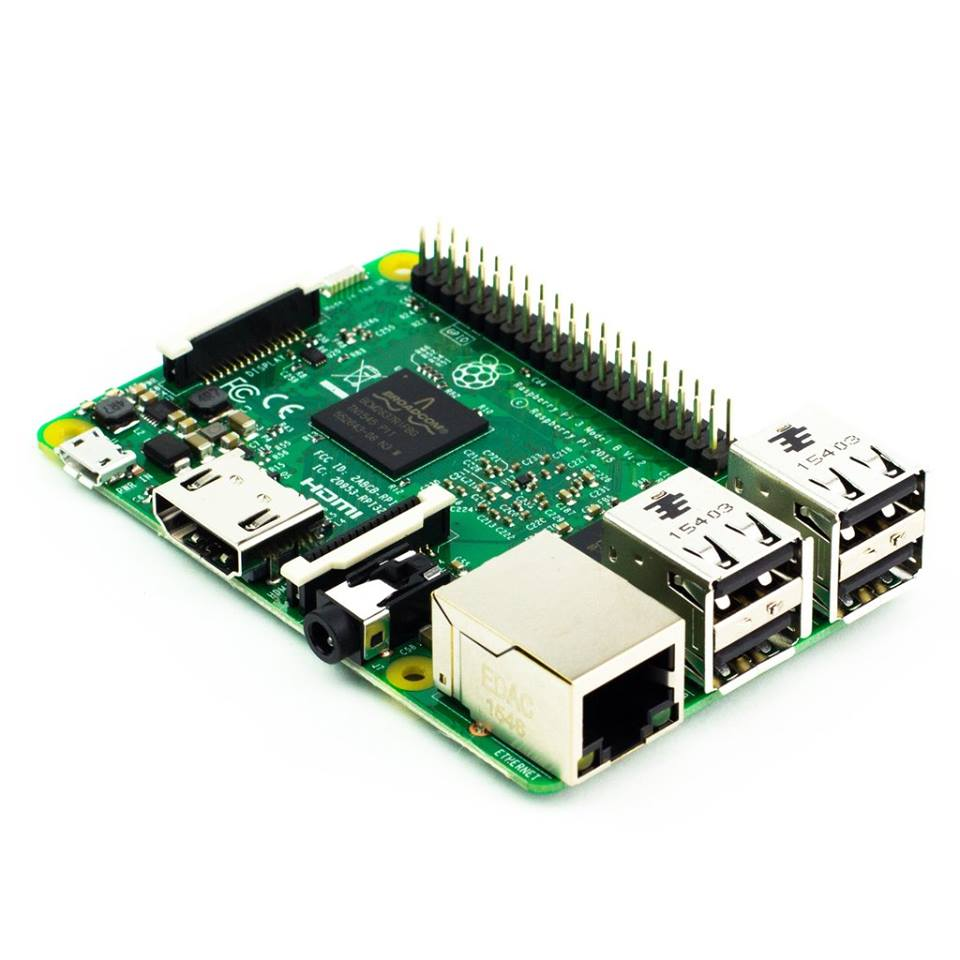
\includegraphics[scale=0.45, angle = 360]{figuras/lala1}
\caption[]{Equipamento Rapberry PI 3}
\end{figure}
\FloatBarrier

\begin{itemize}
\item Raspberry Pi 3 Model B.
\item Processador Broadcom BCM2837 64bit ARMv8 Cortex-A53 Quad-Core.
\item Clock 1.2 GHz.
\item Memória RAM: 1GB.
\item Adaptador Wifi 802.11n integrado.
\item Bluetooth 4.1 BLE integrado.
\item Conector de vídeo HDMI.
\item 4 portas USB 2.0.
\item Conector Ethernet.
\item Interface para câmera (CSI).
\item Interface para display (DSI).
\item Slot para cartão microSD.
\item Conector de áudio e vídeo.
\item GPIO de 40 pinos.
\item Dimensões: 85 x 56 x 17mm.
\end{itemize}

\subsection{Sistema de Controle}

\begin{itemize}
\item{Solução 1: Atuador}
\end{itemize}

Será utilizado um atuador linear (empurra e puxa), fabricado pelos integrantes do grupo (da parte eletrônica), para capturar o livro na estante e levá-lo até o usuário. Na ponta do atuador estará conectado o eletroímã, onde de fato realizará a captura do livro através de sua força eletromagnética. O controle do atuador ficará responsável pela raspberry que terá a incubência de ativa-lo quando chegar no local pretendido. 

\begin{itemize}
\item{Solução 2: Braço Robótico}
\end{itemize}

O braço é a parte da estrutura responsável por agarrar o livro desejado. Como esse sistema irá se movimentar em dois eixos, a padronização dos livros será uma ótima saída. A colocação de cases normalizaria tornando-se mais fácil segurar o livro. O microcontrolador receberia o sinal e apanharia o livro pretendido pelo usuário. Esta estrutura consiste em duas garras que recolheria a case e levaria ao utilizador. Uma enorme parcela da estrutura do braço e do sistema embarcado será executado pela equipe de eletrônica. 

\begin{itemize}
\item{Movimentação do Braço Robótico}
\end{itemize}

O funcionamento do braço será composto basicamente por três partes: microcontrolador, servo motor e modulação PWM. O microcontrolador atmega 2650 (comumente chamado de arduíno MEGA)  estará acoplado junto a base do braço robótico, ele irá controlar o movimento mecânico e a captura do livro. O servo motor é o que realizará a movimentação do braço, girando até 180º dependendo do eixo (x,y,z) em que foi colocado. A modulação PWM ditará a posição da movimentação do braço, ou seja, controlará a abertura do braço para posição desejada (ângulo).

Para a captura do livro foi escolhido o eletroímã, assim o microcontrolador terá que cuidar da parte de acionamento do mesmo, onde só será feito depois de comprovado que o livro pretendido de fato está no local estipulado.

\begin{itemize}
\item{Servo Motor}
\end{itemize}

São destinados e projetados para uso em aplicações de controle de movimento que exigem posicionamento de alta precisão, reversão rápida e desempenho excepcional.Para manter o controle constante entre o arduino e o servo, é necessário usar um servo motor tipo CC, ele será de baixa potência pois a tensão de alimentação é pequena. Seus componentes são:

\begin{itemize}
\item Motor: Acionamento das engrenagens e eixo principal do servo motor.
\item Engrenagens: Redução de rotação do motor e aumento do torque.
\item Encaixe de saída: conexão de saída do motor.
\item Potenciômetro: Monitora a posição do motor.
\item Circuito de controle: Monitora a saída do potenciômetro e a ativação do motor interno para manter a posição determinada na entrada.
\end{itemize}

\begin{figure}[!h]
\centering
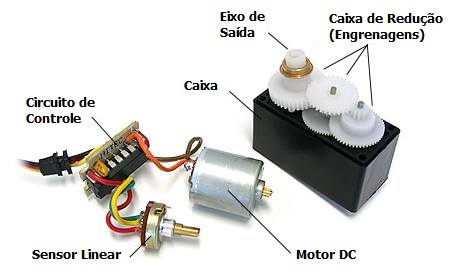
\includegraphics[scale=0.65, angle = 360]{figuras/lala2}
\caption[]{Equipamento Servo Motor}
\end{figure}
\FloatBarrier

\begin{itemize}
\item{Modulaçao PWM}
\end{itemize}

O controle do servo motor é obtido por um sinal de tensão de referência CC, esse sinal é produzido por um gerador de largura de pulso de controle (PWM- Pulse Width Modulation) e servirá para obter a posição angular desejada do motor. Assim com base na figura 1.2 podemos ter a ideia de como funciona. Uma informação é codificada em modulação PWM através da largura do pulso em nível alto em relação ao período total de oscilação, ou seja, através do seu fator de forma (duty cycle).

No PWM tem que ser levado em consideração dois parâmetros, frequência e largura dos pulsos. A frequência é fixa e será gerada pelas saídas digitais do controlador, já a largura varia de tamanho e esse tamanho auxiliará na posição angular do braço.

\begin{figure}[!h]
\centering
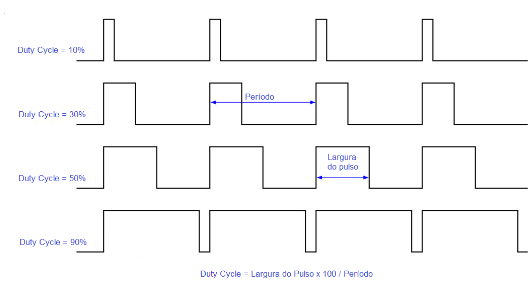
\includegraphics[scale=0.65, angle = 360]{figuras/lala3}
\caption[]{Modulação PWM e fator de forma}
\end{figure}
\FloatBarrier

\begin{itemize}
\item{Arduino MEGA}
\end{itemize}

É o microcontrolador que realizará a parte de controle do braço e acionamento do eletroímã. Ele receberá os comandos da raspberry para executar os movimentos para segurar a case contendo o livro requisitado. Suas especificações são:

\begin{figure}[!h]
\centering
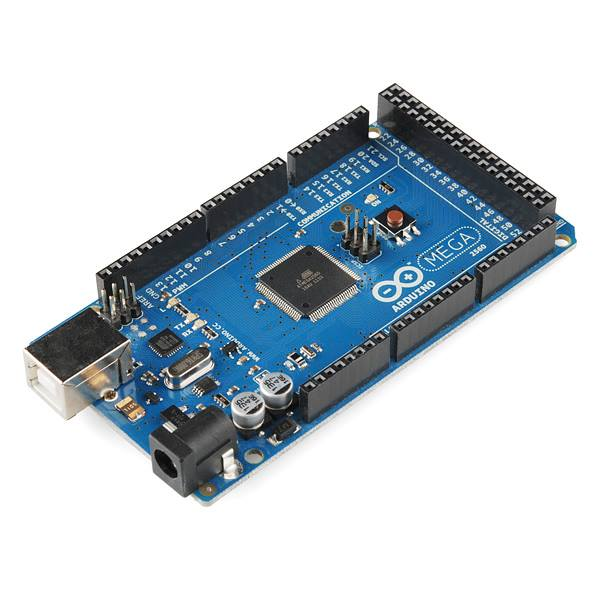
\includegraphics[scale=0.65, angle = 360]{figuras/lala4}
\caption[]{Equipamento Arduino Atmega 2560}
\end{figure}
\FloatBarrier

\begin{itemize}
\item Microcontrolador: ATmega2560.
\item Tensão de Operação: 5V.
\item Tensão de Entrada: 7-12V.
\item Portas Digitais: 54 (15 podem ser usadas como PWM).
\item Portas Analógicas: 16.
\item Corrente Pinos I/O: 40mA.
\item Corrente Pinos 3,3V: 50mA.
\item Memória Flash: 256KB (8KB usado no bootloader).
\item SRAM: 8KB.
\item EEPROM: 4KB.
\item Velocidade do Clock: 16MHz.
\end{itemize}

\begin{itemize}
\item{Solução Escolhida}
\end{itemize}

A solução escolhida será a do atuador, por ser mais fácil a construção, contudo, a solução do braço  não será totalmente descartada a princípio, devido a sua complexidade, pode ser motivada pelo desafio onde aumentará o nível do projeto.

\subsection{Sistema de Comunicação}

\begin{itemize}
\item{Comunicação UART}
\end{itemize}

A UART (Universal Asynchronous Receiver/Transmitter) como o próprio nome já diz é um sistema de comunicação em que dados digitais são transmitidos e recebidos na forma serial operando no modo assíncrono. Neste projeto, a UART estará presente na comunicação entre a Raspberry e o Arduino, onde o usuário irá escolher o livro através de uma página em uma rede local, a rasp então irá traduzir as escolhas feitas na página em comandos para o Arduino via UART. Para isso é necessário tomar alguns cuidados:

\begin{itemize}
\item BAUD RATE(Clock de operação) : Os dois dispositivos devem possuir o mesmo baud rate, caso contrário não funcionará a comunicação, necessário procurar no datasheet do microcontrolador (na sessão da UART) o cálculo do baud rate. A unidade de operação é em bps (bits por segundo).
\item Configuração do protocolo: O protocolo de UART pode ser configurado para mandar dados de 8 ou 9 bits, com possibilidade de bits de paridade (par, ímpar, nenhum), com 1 ou 2 bits de parada. Os dois dispositivos devem possuir a mesma configuração.
\end{itemize}

\begin{itemize}
\item{Leitura do Código de Barras}
\end{itemize}

A leitura do código de barras será feita manualmente pela bibliotecário onde tem como função informar baixa do livro no servidor quando o usuário pegar o livro e quando chegar novos livros à biblioteca ele adiciona no banco de dados. 

\begin{figure}[!h]
\centering
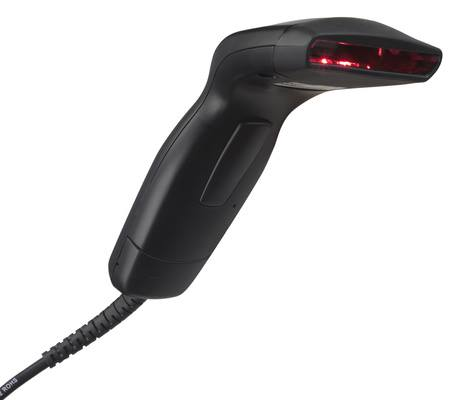
\includegraphics[scale=0.65, angle = 360]{figuras/lala5}
\caption[]{Equipamento leitor de código de barras}
\end{figure}
\FloatBarrier
